% Options for packages loaded elsewhere
\PassOptionsToPackage{unicode}{hyperref}
\PassOptionsToPackage{hyphens}{url}
%
\documentclass[
]{article}
\usepackage{amsmath,amssymb}
\usepackage{iftex}
\ifPDFTeX
  \usepackage[T1]{fontenc}
  \usepackage[utf8]{inputenc}
  \usepackage{textcomp} % provide euro and other symbols
\else % if luatex or xetex
  \usepackage{unicode-math} % this also loads fontspec
  \defaultfontfeatures{Scale=MatchLowercase}
  \defaultfontfeatures[\rmfamily]{Ligatures=TeX,Scale=1}
\fi
\usepackage{lmodern}
\ifPDFTeX\else
  % xetex/luatex font selection
\fi
% Use upquote if available, for straight quotes in verbatim environments
\IfFileExists{upquote.sty}{\usepackage{upquote}}{}
\IfFileExists{microtype.sty}{% use microtype if available
  \usepackage[]{microtype}
  \UseMicrotypeSet[protrusion]{basicmath} % disable protrusion for tt fonts
}{}
\makeatletter
\@ifundefined{KOMAClassName}{% if non-KOMA class
  \IfFileExists{parskip.sty}{%
    \usepackage{parskip}
  }{% else
    \setlength{\parindent}{0pt}
    \setlength{\parskip}{6pt plus 2pt minus 1pt}}
}{% if KOMA class
  \KOMAoptions{parskip=half}}
\makeatother
\usepackage{xcolor}
\usepackage[margin=1in]{geometry}
\usepackage{graphicx}
\makeatletter
\def\maxwidth{\ifdim\Gin@nat@width>\linewidth\linewidth\else\Gin@nat@width\fi}
\def\maxheight{\ifdim\Gin@nat@height>\textheight\textheight\else\Gin@nat@height\fi}
\makeatother
% Scale images if necessary, so that they will not overflow the page
% margins by default, and it is still possible to overwrite the defaults
% using explicit options in \includegraphics[width, height, ...]{}
\setkeys{Gin}{width=\maxwidth,height=\maxheight,keepaspectratio}
% Set default figure placement to htbp
\makeatletter
\def\fps@figure{htbp}
\makeatother
\setlength{\emergencystretch}{3em} % prevent overfull lines
\providecommand{\tightlist}{%
  \setlength{\itemsep}{0pt}\setlength{\parskip}{0pt}}
\setcounter{secnumdepth}{5}
\usepackage[german]{babel}
\usepackage{mathtools}
\usepackage{tikz}
\usepackage{pgf}
\usepackage{csquotes}
\AtBeginDocument{
\renewcommand{\maketitle}{}
}
\PassOptionsToPackage{a4paper,margin = 2.5cm}{geometry}
\usepackage{geometry}
\usepackage{float}
\usepackage{enumitem}
\newcommand{\bcenter}{\begin{center}}
\newcommand{\ecenter}{\end{center}}
\renewcommand{\contentsname}{Inhalt}
\usepackage{blindtext}
\usepackage[backend=biber, style = apa]{biblatex}
\addbibresource{Literatur.bib}
\usepackage{multirow}
\usepackage{booktabs}
\usepackage{array}
\usepackage{pdflscape}
\usepackage{afterpage}
\ifLuaTeX
  \usepackage{selnolig}  % disable illegal ligatures
\fi
\usepackage[]{biblatex}
\addbibresource{Literatur.bib}
\usepackage{bookmark}
\IfFileExists{xurl.sty}{\usepackage{xurl}}{} % add URL line breaks if available
\urlstyle{same}
\hypersetup{
  pdftitle={Hausarbeit},
  pdfauthor={Franz Andersch \& Niklas Münz},
  hidelinks,
  pdfcreator={LaTeX via pandoc}}

\title{Hausarbeit}
\author{Franz Andersch \& Niklas Münz}
\date{2024-08-26}

\begin{document}
\maketitle

\begin{titlepage}
	\begin{center}
		
		
\includegraphics[width=0.5\textwidth]{images/UB-Logo-blau.png}
		
		\LARGE
		\textbf{Otto-Friedrich Universität Bamberg}\\
		\textbf{Lehrstuhl für Statistik und Ökonometrie}\\
		\textbf{Statistical Machine Learning}
		
		
		\vspace*{1.5cm}
		
		\Huge
		\textbf{Unser Thema}
		
		
		\vspace{2cm}
		
		\Large
		\begin{minipage}[t]{0.4\textwidth}
			\textbf{Autoren:}
		\end{minipage}
		\hfill
		\begin{minipage}[t]{0.3\textwidth}
			Niklas Münz\newline
			Matrikel Nr.: 2150715
			
			\vspace{0.3cm}
			
			Franz Andersch\newline
			Matrikel Nr.: 2154877
			
		\end{minipage}
		
		\vspace{0.5cm}
		
		\Large
		\begin{minipage}[t]{0.4\textwidth}
			\textbf{Studiengang:}
		\end{minipage}
		\hfill
		\begin{minipage}[t]{0.3\textwidth}
			MSc. Survey Statistics \newline
			\& Data Analysis
		\end{minipage}
		
		\vfill
		Sommersemester 2024
		
	\end{center}
\end{titlepage}
\newpage
\tableofcontents
\thispagestyle{empty}
\clearpage
\pagenumbering{arabic}
\section{Einleitung}

Warum eine gerade Ebene manchmal die beste Möglichkeit ist, um Daten in
zwei klassen aufzuteilen? Darum soll es in dieser Arbeit gehen. Wir
wollen hier die Methode der Support Vector Machines, die mit dieser
Annahme arbeitet, erläutern und gleichzeitig auf den Prüfstand stellen.
Denn auch wenn die Grundidee, vielleicht etwas zu simpel klingt, ist
ihre Leistung was vor allem binäre Klassifikationprobleme angeht
unumstritten. Die Grundlage für eine optimal seperierende Hyperebene
wurde bereits 1964 von Alexej Chervonenkis und Vladimir Vapnik gelegt
und die Methode wurde anschließend von mehrern Autoren stetig erweitert
\parencite{vapnikEstimationDependencesBased2006}. Zuerst wollen wir die
Funktionsweise der SVM näher beleuchten. Dazu wird zuerst gezeigt wie
die Konstruktion dieser seperiernden Hypereben in dem Fall funktioniert,
in dem die Daten tasächlich linear trennbar sind. Danach soll gezeigt
werden wie eine Soft Margin Klassifier funktioniert, der auch
funktioniert bei nicht perfekt linear trennbaren Daten und zuletzt soll
es um die Anwendung von Kernels gehen, die es dann auch ermöglichen,
nicht lineare Entscheidungsgrenzen herzustellen. im Kapitel 3 wollen wir
dann die Vor und Nachteile der Methode uns anschauen. Anhand dieser
Informationen konnten wir uns dann bereits einige Gedanken zur Leistung
der SVM in unserem Datenexperiment machen. Wie wir dieses Experiment
aufbauen soll im nachfolgenden Kapitel beschrieben werden. Wir
generieren uns zum anschließenden Vergleich neun verschiedene
Datenszenarien, welche in ihrer Dimensionalitäten und Kompleixität der
Entscheidungsgrenze variieren. Für den Vergleich wollen wir dann
Klassifikationsleistung von SVM uns anderen Klassifikationsmethoden
vegleichen. Im Teil Hypothesen haben wir aufgrund von Literatur, die
bereits ähnliche Versuche durchgeführt haben, Vermutungen aufgestellt,
wie die einzelnen Classifier im Vergleich abschneiden werden. Im
Ergebnis-Teil wollen wir dann das Experiment durchführen und mithilfe
von verschiedenen Maßzahlen die Leistung evaluieren. Ebenfalls wollen
wir üperprüfen, ob die Hypothesen die wir zuvor aufgestellt haben sich
bewahrheiten. Im letzen Teil soll ein Fazit gezogen werden, in dem Wir
die Ergebnisse noch einmal diskutieren und Defitite in unserer Arbeit
aufarbeiten.

\section{Funktionsweise}

\subsection{Hard Margin Classifier}

Um das grundlegende Prinzip der SVMs darzustellen gehen wir zuerst von
einer Datensituation aus, in der sich zwei gruppen optimal durch eine
lineare entscheidungsgrenze trennen lassen. Das endgültige Ziel ist es
eine sogenannte Hyperplane zu finden die diese Daten möglichst gut
seperiert und als Entscheidungsgrenze funktioniert. Die allgemeine Form
einer solchen hyperplain lautet \begin{align}
\beta_0+ \beta_1 X_1+\beta_2 X_2+...+\beta_n X_n=0\label{eq:hyperebene}
\end{align} oder in Vektorschreibweise \begin{align}
\overline{\beta}\cdot\overline{x}+\beta_0=0 \label{eq:hyperplanevec}
\end{align} Die geometrische Interpretation des Vektors \(\beta\) und
des Skalars \(\beta_0\) wird in Abbildung \ref{fig:Ebene} im zwei
dimensionalen Fall dargestellt.

\begin{figure}[htb]
    \centering
    \begin{minipage}{0.45\textwidth} 
        \centering
        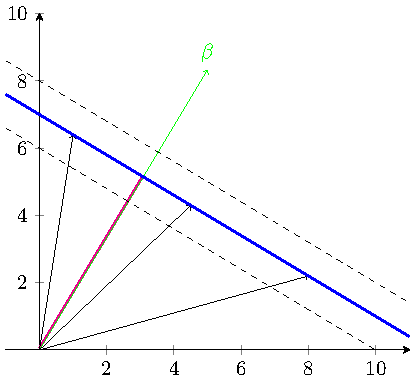
\includegraphics[width=\textwidth,trim=0.5cm 0.5cm 0.5cm 0.5cm]{Images/decision_boundary.pdf} 
        \caption{Konstruktion der Hyperebene}
        \label{fig:Ebene}
    \end{minipage}\hfill
    \begin{minipage}{0.45\textwidth} 
        \centering
        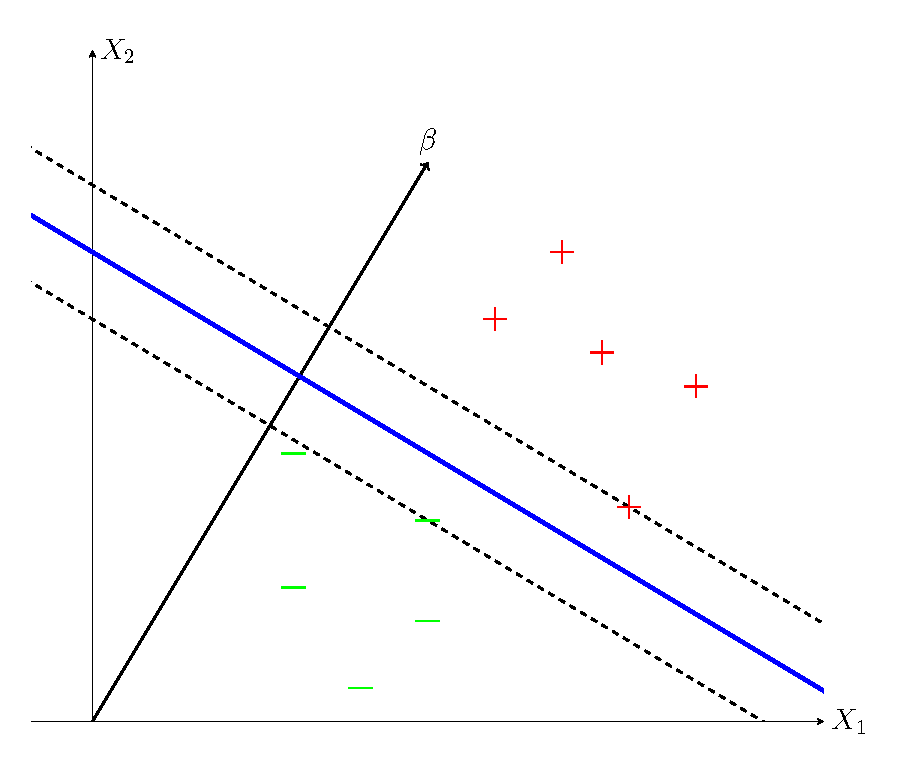
\includegraphics[width=\textwidth,trim=0.5cm 0.5cm 0.5cm 0.5cm]{Images/guttes.pdf}
        \caption{Konstruktion der Margins}
        \label{fig:Margin}
    \end{minipage}
\end{figure}

Die blaue Linie soll die Hyperplain darstellen. Im zweidiemnsionalen
handelt es sich hier um eine Linie. Der \(2 \times 1\) Vektor
\(\overline{\beta}\) liegt immer senkrecht zur konstruierten Hyperplane.
Würde man alle Vektoren, die auf der Hyperplane landen, auf den
\(\overline{\beta}\)-Vektor Projezieren, dann hätten alle diese
Projektionen die selbe Länge \(c\). Also gilt für alle Punkte, die auf
der Ebene liegen. \begin{align}
\frac{\overline \beta}{||\overline{\beta}||}\cdot \overline{x}=c \Leftrightarrow \overline{\beta}\cdot \overline{x}=c \cdot ||\overline{\beta}||\label{eq:betanull}
\end{align} ersetzet man in \eqref{eq:betanull}
\(c \cdot ||\overline{\beta}||\) mit \(-\beta_0\) und zieht dies dann
auf die andere Seite, kommen man wieder bei der ursprünglichen Form aus
Formel \eqref{eq:hyperplanevec} raus.

Als nächstes stellt sich jetzt die Frage, welches \(\overline{\beta}\)
und \(\beta_0\) die optimale Hyperplane darstellen. Betrachtet man die
Abbildung \ref{fig:Margin}, dann ist zu erkennen, dass die Datenpunkte
durch die blaue Linie getrennt werden. Allerdings könnte man
theorethisch undendlich viele andere Hyperplains durch rotation oder
verschiebung konstruieren, die trotzdem die Daten in ihren Ausprägungen
trennen. Um eine eindeutige Lösung zu finden, wird als nächstes ein
bereich um die Hperplane abgesteck. In Abbildung \ref{fig:Margin}
dargestell durch die gestrichelten scharzen linien, welche man als
Schranken bezeichnen könnte. In diesem Bereich sollen keine Datenpunkte
liegen und die Schranken sollen immer parallel zur Hyperplain seien und
den gleichen Abstand zu ihr haben. Außerdem dürfen keine positiven
Samples unterhalb der oberen Schranke liegen und keine negativen
unterhalb. Das gegenteil gilt dementsprechend für die untere Schranke.
Als Definition für die beiden Schranken wird festgelegt \begin{align}
\overline{\beta}\cdot \overline{x}+\beta_0=1\label{eq:posSV}
\end{align} für die Schranke in richtung der grünen Datenpunkte und
\begin{align}
\overline{\beta}\cdot \overline{x}+\beta_0=-1\label{eq:negSV}
\end{align} für die Schranke in Richting der roten Datenpunkte. Aus
dieser Beschränkung für die Hyperplane können wir auch ableiten, dass
für die positiven Samples \(\overline{x}^+\) immer gilt
\(\overline{\beta}\cdot \overline{x}^++\beta_0\ge 1\) und für negative
Samples \(\overline{x}^-\) immer gilt
\(\overline{\beta}\cdot \overline{x}^-+\beta_0\le -1\). Durch einführen
einer weiteren Variable \(y\), welche die eigenschaft hat, dass die den
Wert 1 bei einem positiven und den Wert -1 bei einem negativen Sample
annimmt, können diese zwei Beschränkungen zu einer zusammengefasst
werden \begin{align}
y_i(\overline{\beta}\cdot \overline{x}_i+\beta_0)\ge 1\label{eq:Nebenbedingung}
\end{align} Da das Verfahren auch maximum Margin Classifier gennant
wird, gilt es jetzt noch eine Definition für den Margin also den Abstand
zwischen den zwei Schranken zu finden, der schließlich maximiert werden
soll. Damit diese Schranken, maximal weit auseinander liegen, muss es
zwangsläufig Datenpunkte geben, die genau auf den Schranken liegen.
Diese Datenpunkte haben eine wichtige Rolle für die Konstruktion des
Margins. Es sind ausschließlich diese Datenpunkte, die einen Einfluss
auf die finalen werte von \(\overline{\beta}\) und \(\beta_0\) haben
werden. Sie werden \textbf{Support-Vektoren} genannt und geben den SVMs
ihren Namen.

\begin{figure}[htb]
\centering
 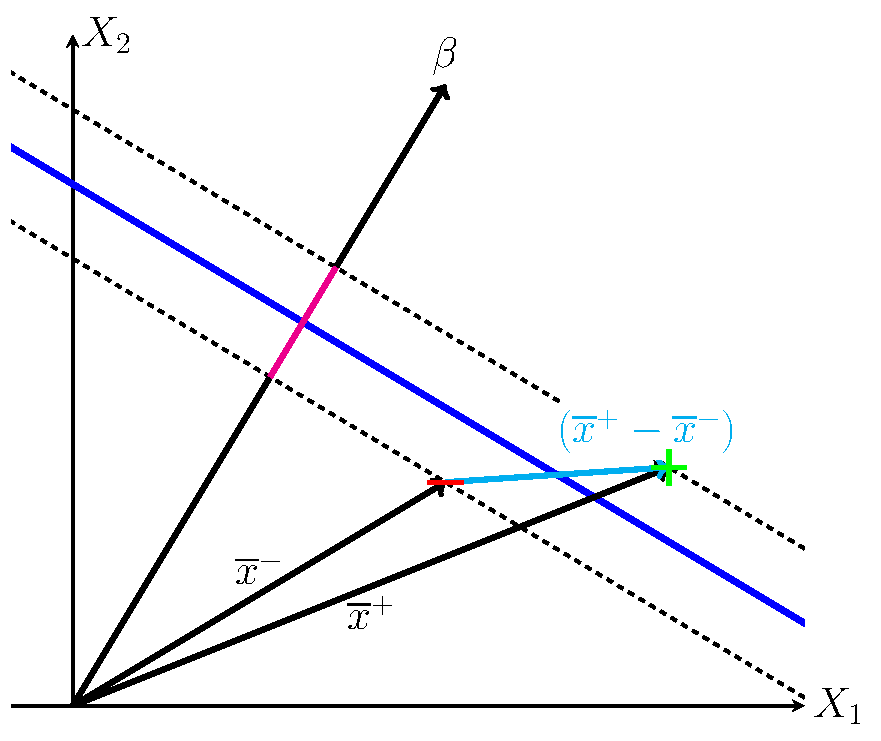
\includegraphics[width=0.5\textwidth,trim=0.5cm 0.5cm 0.5cm 0.5cm]{Images/margin.pdf} 
        \caption{Abhängigkeit des Margins von den Support-Vektoren}
        \label{fig:SupVecs}
\end{figure}

In Abbildung \ref{fig:SupVecs} sind zwei solcher Support-Vektoren zu
einem negativen und positiven Sample dargestellt. Der Margin kann dann
dargestellt werden als eine Projektion dieser Differenz
(\(\overline{x}^+-\overline{x}^+\)) auf den \(\overline{\beta}\)-Vektor.
Damit am Ende die Länge dieses Margins \(M\) rauskommt muss
\(\overline{\beta}\) noch durch seine Länge geteilt werden.
\begin{align}
M=\frac{\overline{\beta}}{||\overline{\beta}||}\cdot \left(\overline{x}^+-\overline{x}^+\right)=\frac{\overline{\beta}\cdot\overline{x}^- -\overline{\beta}\cdot\overline{x}^+}{||\overline{\beta}||}\label{eq:maring1}
\end{align} Es ist bekannt, dass für postive Supportvektoren gilt
\(\overline\beta \overline{x}^+ +\beta_0 = 1 \Leftrightarrow \overline\beta \overline{x}^+=1-\beta_0\)
und für negative
\(\overline\beta \overline{x}^- +\beta_0 = -1 \Leftrightarrow \overline\beta \overline{x}^-=-1-\beta_0\).
Setzt man dies ein in \eqref{eq:maring1}, erhält man als
Maximisierungsziel \begin{align}
M=\frac{1-\beta_0-(-1-\beta_0)}{||\overline\beta||}=\frac{2}{||\overline\beta||}\label{eq:margin2}
\end{align} Um diesen Maximierungsschritt angenehmer zu gestalten, wird
an der Stelle versucht den Ausdruck
\(\frac{1}{2}||\overline \beta||^2=\frac{1}{2}\overline \beta '\cdot \overline \beta\)
zu minimieren. Was im Endeffekt ebenfalls dazu führt, dass der Ausdruck
in \eqref{eq:margin2} maximiert wird.

Dieses Optimierungsproblem mit der Nebenbedingung aus Formel
\eqref{eq:Nebenbedingung} lässt sich am besten über Lagrange-Multiplier
lösen \begin{align}
\mathcal{L}(\overline\beta,\beta_0,\overline \alpha)=\frac{1}{2}\overline \beta ' \overline \beta-\sum \alpha_i[y_i(\overline \beta \cdot \overline{x_i}+\beta_0)-1]\label{eq:Lagrange}
\end{align} Wird dieser Ausdruck partiell abgeleitet und gleich null
gesetzt erhält man als zwischen ergebnis \begin{align}
\frac{\partial \mathcal{L}}{\partial \beta}=\beta-\sum \alpha_i y_i \overline{x_i}\overset{!}{=}0 \Rightarrow \beta=\sum \alpha_i y_i \overline{x_i}\label{eq:solutbeta}
\end{align} somit zeigt sich, dass \(\overline{\beta}\) als
linearkombination der Inputvektoren dargestellt werden kann. Weiterhin
gilt für \(\beta_0\) \begin{align}
\frac{\partial \mathcal{L}}{\partial \beta_0}=\sum \alpha_i y_i \overline{x_i}\overset{!}{=}0\label{eq:solutbeta0}
\end{align} Setzt man dies in \eqref{eq:Lagrange} ein erhält man einen
neuen Ausdruck, denn es gilt zu minimieren \begin{align}
\mathcal{L}(\overline \alpha)=-\frac{1}{2}\sum \sum \alpha_i \alpha_j y_i y_j \overline{x}_i \cdot \overline{x}_j+\sum \alpha_i\label{eq:dualproblem}
\end{align} Die Lösung für diesen Ausdruck erfolgt dann über sogenannte
\enquote{standard non linear optimization algorithms for quadratic forms}
\parencite{boserTrainingAlgorithmOptimal1992}. Nachem für
\(\overline \alpha\) gelöst wurde, kann dies in \eqref{eq:solutbeta}
eingesetzt werden um das optimale \(\overline{\beta}\) zu erhalten. Es
kann gezeigt werden, dass die gelösten \(\alpha_i\) lediglich für die
Supportvektoren werte ungelich Null annehmen. Somit ist der
Koeffizientenvektor \(\overline{\beta}\) sogar eine Linearkombination
von nur den Supportvektoren
\parencite{boserTrainingAlgorithmOptimal1992}. Die letzte unbekannte
\(\beta_0\) kann gelöst werden, indem man mithilfe von einem
positiven/negativen Support Vektor \eqref{eq:posSV}/ \eqref{eq:negSV}
nach \(\beta_0\) löst.

Mit den gelösten Werten zur optimalen Hyperplane kann jetzt auch eine
Entscheidungsregel für ungelabelte Datenvektoren \(\overline{x}_u\)
konstruiert werden. Bedenkt man also wenn man einen Vektor der nicht auf
der Hypeplane liegt in \eqref{eq:betanull} einsetzt erhält man also
\(\frac{\overline \beta}{||\overline{\beta}||}\cdot \overline{x}_u=c+k\).
Wenn \(k\) positiv ist, liegt der neue Datenpunkt oberhalb der
Hyperplane liegt und somit als positives Sample gewertet wird. Wenn
\(k\) negativ ist, dann liegt der Datenpunkt unterhalb der Hyperplane
und wird als negativ gewertet. Mit der gleichen Umformung wie weiter
oben schon beschrieben kommt man zu folgender Entscheidungsregel
\begin{align}
f(\overline{x}_u)=\begin{cases}\mathrm{positiv}&\text{wenn } \overline{\beta}\cdot \overline{x}_u+\beta_0 > 0\\
\mathrm{negativ} & \text{wenn }\overline{\beta}\cdot \overline{x}_u+\beta_0<0
\end{cases}\label{eq:decisionf}
\end{align}

\subsection{Soft Margin Classifier}

Dass die Daten sich perfekt linear trennen lassen ist zwar ein gut um
die Vorgehensweise zu veranschaulichen, tritt aber in realen Situationen
so gut wie nie auf. Falls sich postitive und negative Samples im Raum
überlappen, ist die Konstruktion einer Hyperplane wie beim Hard Margin
Classifier unmöglich. Man müsste also entweder auf eine nicht lineare
Hypeplane ausweichen oder man erweicht die vorgaben für die Konstruktion
der Hyperplane. Zweiteres ist genau das, was durch die Soft Margin
Classifier erreicht wird. Die Vorgabe für die Konstruktion der Schranken
ermöglicht es einzelnen Datenpunkten auf der falschen Seite der
Schranke, ja sogar der Entscheidungsgrenzen zu liegen. Dafür wird für
die Einschränkungen eine sogennannte Slackvariable \(\varepsilon\)
eingeführt \parencite{jamesIntroductionStatisticalLearning2021}. Setzt
man diese in diese in \eqref{eq:Nebenbedingung} lautet die neuen
Nebenbedingung \begin{align}
y_i(\beta \cdot \overline{x}_i-\beta_0)>1- \varepsilon_i \label{eq:nebbedsfm}
\end{align}

\begin{figure}[htb]
\centering
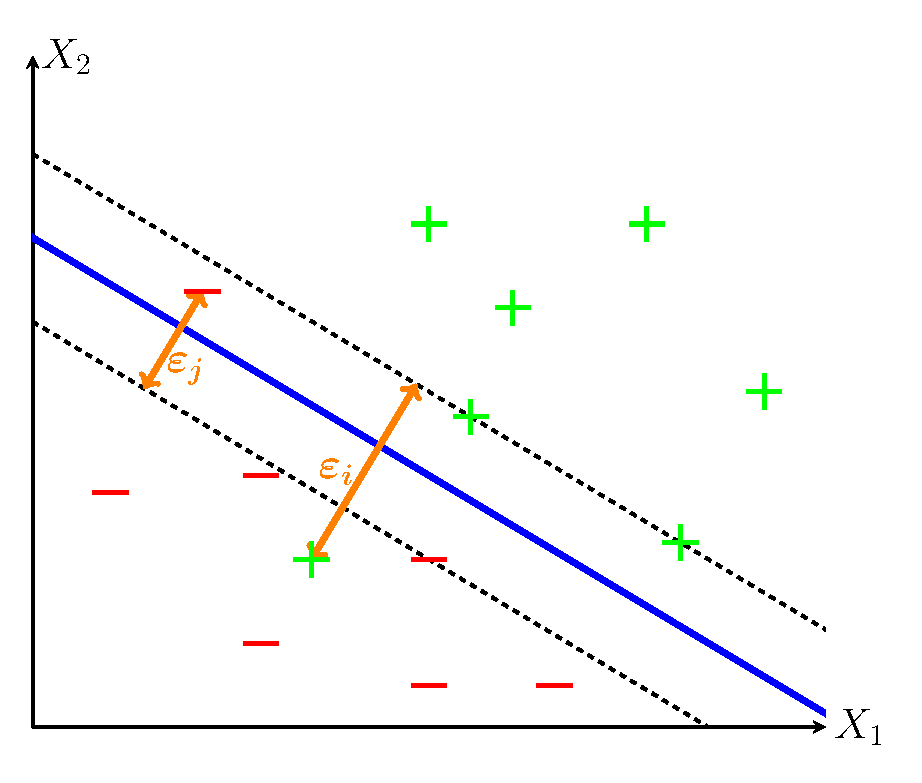
\includegraphics[width=0.5\textwidth,trim=0.5cm 0.5cm 0.5cm 0.5cm]{Images/slackvariable.pdf} 
        \caption{Funktion der Slack Variable}
        \label{fig:slackvariable}
\end{figure}

Jetzt könnte man versuchen diese neue Nebenbedingung einfach in das
zuvor angewandte Optimisierungsverfahren einzufügen. Allerdings besteht
hier das Problem, dass \(\varepsilon\) einfach immer maximal groß
gewählt wird und so die Bedingung immer erfüllt wird. Um das Ausmaß der
Verletzung der usptünglichen Annahmen zu begrenzen, aber trotzdem noch
gewisse Abweichung zuzulassen, wird ein weitere Parameter \(C\)
eingeführt, als regularisierender Parameter für \(\varepsilon\). Leitet
daraus zusammen mit der Restriktion \(\varepsilon\ge0\) wieder einen
Lagrangefunktion her erhält man \begin{align}
\mathcal{L}(\overline\beta,\beta_0,\overline\alpha,\overline\varepsilon,\overline\lambda)=\frac{1}{2}\overline\beta'\cdot \overline\beta + C \sum_{i=1}^{n}\varepsilon_i-\underbrace{\sum \alpha_i[y_i(\overline\beta \cdot \overline{x_i}+\beta_0)-1+\varepsilon_i]}_{\text{für }y_i(\overline\beta \cdot \overline{x}_i-\beta_0)>1- \varepsilon_i}-\underbrace{\sum \lambda_i \varepsilon_i }_{\substack{\text{für}\\ \varepsilon_i \ge 0}}
\end{align} Wenn dieser Ausdruck wie beim Hardmargin Classifier gelöst
wird und die Ergebnisse eingesetzt werden erhält man wieder den Ausruck
aus \eqref{eq:dualproblem} mit der zusätzlichen Einschränkung
\(0\le \alpha_i \le C\). Dieses Maximierungsproblem wird dann genauso
aufgelöst wie bei dem Hard Margin Classifier und die Entscheidungsregel
ist ebenfalls gleich.

\subsection{Der Kernel Trick}

Auch wenn eine lineare Entscheidungsgrenze Vorteile in Sachen
Generalisierbarkeit bietet, ist sie doch nicht für jede Datensituation
geeignet.In Abbildung \ref{fig:nonlinearsep} ist es sehr gut zu
erkennen, dass in diesem Fall eine lineare Grenze zwischen den Klassen
keinen Sinn Ergeben würde und eine elliptische Form wahrscheinlich
besser geeignet wäre. Eine Lösung für dieses Problem, wäre den
Merkmalsraum zu erweitern. So könnte die angenommene Formel für die
lineare Hyperebene in \eqref{eq:hyperebene} durch polynomterme der
Merkmale \(X_i\) oder durch Interaktionstherme erweitert werden. Dies
führt dazu, dass die Entscheidungsgreze in diesem vergrößerten
Merkmalsraum immer noch linear ist, aber die Trennung möglich ist (siehe
Abbildung \ref{fig:featurexten}). Transformiert man diese dann wieder in
den ursprünglichen Merkmalsraum ist die Entscheidungsgrenze dann nicht
mehr linear. Allerdings führt diese Herangehensweise zu eine starken
Anstieg des Rechenaufwands, da die Möglichkeiten der Merkmalserweiterung
endlos sind \parencite{jamesIntroductionStatisticalLearning2021}.

Die Lösung für das Problem sind sogenannte Kernel Funktionen. Betrachtet
man die entscheidungsfunktion \eqref{eq:decisionf} und setzt für
\(\overline{\beta}\) die Gleichung aus \eqref{eq:solutbeta} erhält man
\begin{align}
f(x_u)= \sum \alpha_i y_i x_i \cdot x_u +\beta_0
\end{align} Es zeigt sich also, dass die Entscheidungsfunktion im
Wesentlichen aus einer Linearkombiantion von Punktprodukten aus dem
Vektor \(x_u\) mit allen Trainingsvektoren \(x_i\) ergibt. Diese
Punktprodukt kann als Ähnlichkeitsmaß zwischen dem neuen Datenpunkt und
dem jeweiligen Trainingsdatenpunkt interpretiert werden. Es ist nun
Möglich diese Produkte durch eine Funktion zu ersetzen, welche die
Ähnlichkeiten von Datenpunkten anders bewertet. Diese sogenannte Kernel
Funktion \(K(x_i,x_j)\) ermöglicht es eine flexiblere
Entscheidungsgrenze zu implementieren. Der Vorteil ist dabei, dass die
Kernel Funktion nur auf alle Punktprodukte angewndet wird und es dabei
nicht nötig ist den Merkmalsraum zu Erweitern, was wiederum Rechenzeit
spart\parencite{jamesIntroductionStatisticalLearning2021}. Die
Entscheidungsfunktion wird dann mithilfe dieser Kernelfunktionen
berechnet: \begin{align}
  f(x_u)=\sum \alpha_i y_i K(x_i,x_u)+\beta_0
\end{align}

\begin{figure}[htb]
    \centering
    \begin{minipage}{0.45\textwidth} 
        \centering
        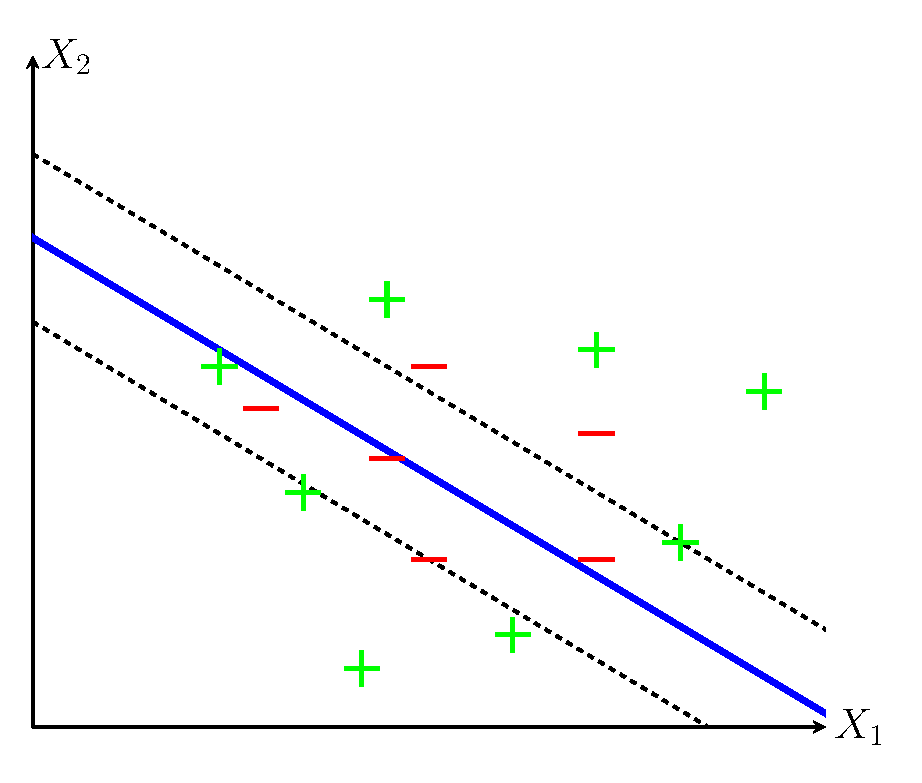
\includegraphics[width=\textwidth,trim=0.5cm 0.5cm 0.5cm 0.5cm]{Images/nonlinearseperable.pdf} 
        \caption{nicht linear getrennte Daten}
        \label{fig:nonlinearsep}
    \end{minipage}\hfill
    \begin{minipage}{0.45\textwidth} 
        \centering
        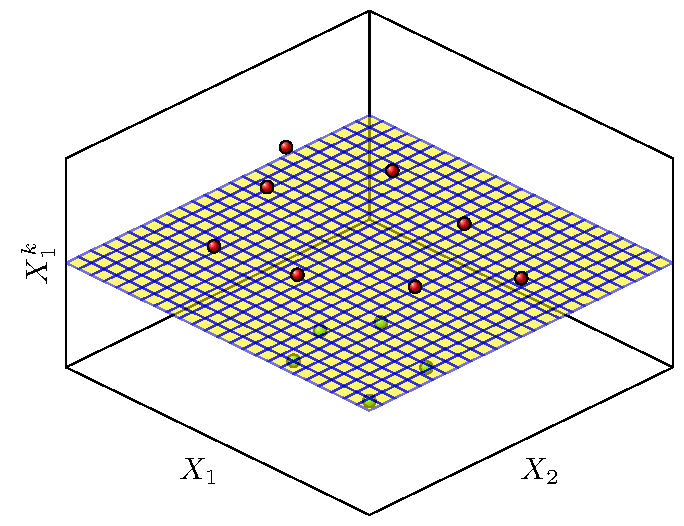
\includegraphics[width=\textwidth,trim=0.5cm 0.5cm 0.5cm 0.5cm]{Images/featurexpansion.pdf}
        \caption{Feature Erweiterung}
        \label{fig:featurexten}
    \end{minipage}
\end{figure}

Es gibt eine ganze Reihe an Kernelfunktionen, die bei SVMs Anwedung
finden. Die Grundlage ist der lineare Kernel, wobei dieser lediglich das
Punktprodukt beschreibt, also praktisch genau das macht, was bei einer
linearen Entscheidungsgrenze gemacht wird. Deweiteren gibt es den
Polynomial Kernel. Dieser hat die Form \begin{align}
 K(x_i,x_u)=(1+x_i\cdot x_u)^d
\end{align} Die Verwendung von diesem Kernel führt dazu, dass die
Entscheidungsgrenze sich ähnlich Verhält, wie als würde man zu Beginn
eine Merkmalserweiterung mit Polynomen vom Grad \(d\) durchführen (siehe
Abbildung \ref{fig:polykernel}. Eine weitere Kernel Funktion ist der
Radial Basis Function Kernel(RBF) mit der Form \begin{align}
K(x_i,x_u)=\exp\left(-\gamma ||x_i-x_u||^2\right)
\end{align} Für diesen Kernel wird die quadrierte euklidische Distanz
als Ähnlichkeitsmaß verwendet, was dazu führt, dass für diejenigen
\(x_i\) die näher an \(x_u\) liegen, in der Entscheidungsfunktion einen
größeren Einfluss haben. Der Parameter \(\gamma\) legt dann fest, wie
stark der Einfluss der Distanz sein soll. Die projektion die der Kernel
hier macht ist eine, in einen uendlich großen Merkmalsraum . Daher
könnte man selbst durch vorgeriges Erweitern des Merkmalsraums nicht das
Ergebnis eines RBF Kernel replizieren und dies führt auch zu einer sehr
flexiblen Entscheidungsgrenze (siehe Abbildung \ref{fig:radialkernel})\\

\begin{figure}[htb]
    \centering
    \begin{minipage}{0.45\textwidth} 
        \centering
        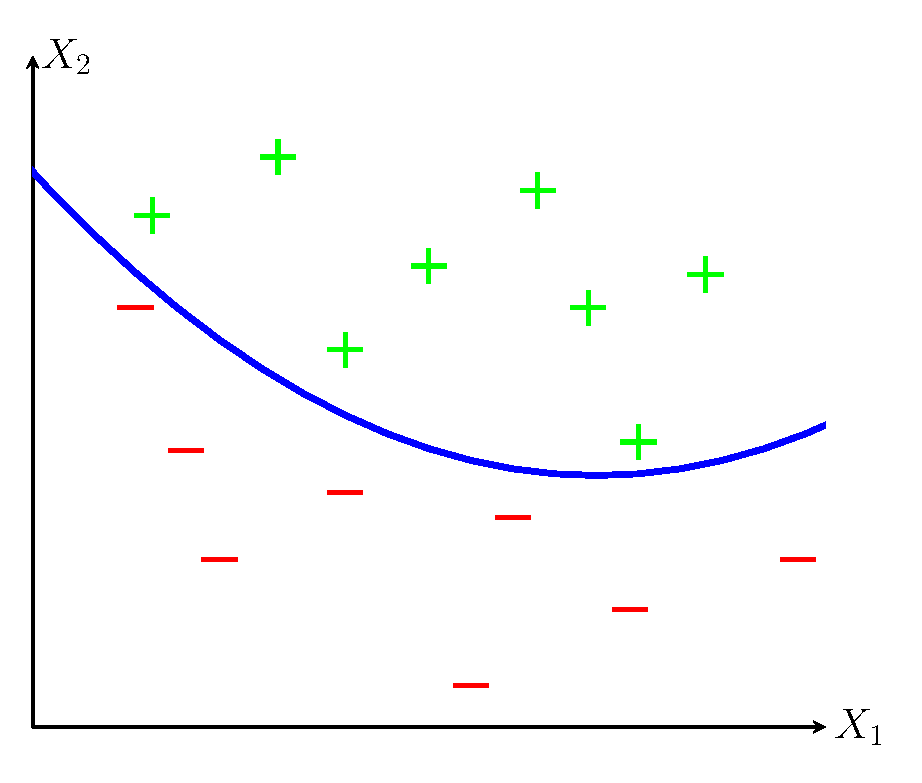
\includegraphics[width=\textwidth,trim=0.5cm 0.5cm 0.5cm 0.5cm]{Images/ploynomial kernel.pdf} 
        \caption{Mögliche Entscheidungsgrenze für polynomial Kernel}
        \label{fig:polykernel}
    \end{minipage}\hfill
    \begin{minipage}{0.45\textwidth} 
        \centering
        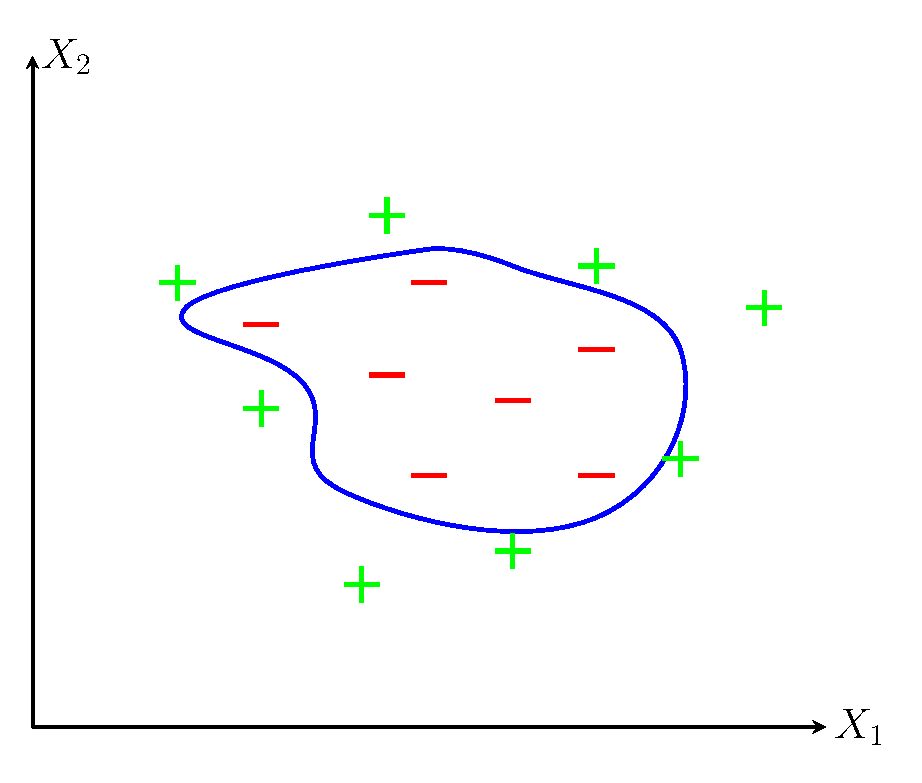
\includegraphics[width=\textwidth,trim=0.5cm 0.5cm 0.5cm 0.5cm]{Images/radial_kernel.pdf}
        \caption{Mögliche Entscheidungsgrenze für RBF Kernel}
        \label{fig:radialkernel}
    \end{minipage}
\end{figure}

Es gibt noch einen Reihe wietere Kernel, die auf unterschiedlichen
Ähnlichkeitsmaßen beruhen, aber eher seltener oder nur in speziellen
Zusammenhänge angewendet werden. Wichtig ist anzumerken, dass die
Verwendung von Kernels zwar die Flexibilität der Entscheidungsgrenze
erhöht, damit aber auch die Gefahr von overfitting einhergeht.
Zusätzlich werden mit den Kernels auch neue Hyperparameter wie \(d\)
oder \(\gamma\) eingeführt, die bei der Model selektion ebenfalls
beachtet werden müssen.\\

\section{Vor- und Nachteile der Methode}

Support Vector Machines haben ein hohes Ansehen unter den Machine
Learning Algorithmen, da sie einige Vorteile mit sich bringen. Aufgrund
der Idee einer Soft Margin und des ``Kernel Tricks'' ist die Methode
sehr flexibel und kann für spezielle Anwendungsbereiche angepasst werden
\parencite{bennettSupportVectorMachines2000}.Dazu sind die Ergebnisse
stabil und reproduzierbar, was sie von anderen Methoden wie
beispielsweise Neural Networks abhebt. Auch die Anwendung ist
vergleichsweise einfach, da es eine überschaubare Anzahl an Parametern
gibt (wie beispielsweise bei der SVM mit radialem Kern nur der gamma-
und cost-Parameter festzulegen ist).\newline Durch die Möglichkeit der
Nutzung verschiedener Kerne sind SVM´s überaus vielseitig. Die Auswahl
des Kerns ermöglicht es äußerst flexible Entscheidungsgrenzen zu formen
\parencite{kuhnAppliedPredictiveModeling2013}. Dadurch können SVM´s an
verschiedene Datensituationen angepasst werden.\newline Ein weiterer
Vorteil ist, dass die Methode weitgehend robust gegenüber overfitting
ist \parencite{kuhnAppliedPredictiveModeling2013}. Dafür verantwortlich
ist der Cost-Parameter, anhand dessen der Fit an die Daten kontrolliert
werden kann. Jedoch birgt dies auch Probleme (Erläuterungen im folgenden
Abschnitt).\newline Diese Vorteile resultieren in einer allgemein
häufigen Nutzung von SVM´s in der Wissenschaft. Sie haben folglich
bewiesen, dass sie für verschiedenste Aufgaben gut funktionieren
\parencite{kuhnAppliedPredictiveModeling2013}.

Trotz der vielfachen Nutzung von SVM´s, bringen sie auch Nachteile mit
sich. Das wohl größte Problem liegt in der Modellselektion
\parencite{bennettSupportVectorMachines2000}. Wie bereits im vorherigen
Abschnitt erwähnt, ist die Auswahl der Parameter von hoher Bedeutung bei
der Performance und dem Fit an die Daten. So kontrollieren die
Kernspezifischen Parameter und der Cost-Parameter einerseits die
Komplexität und andererseits den Fit an die Daten
\parencite{kuhnAppliedPredictiveModeling2013}. Dabei kann die Wahl der
Parameter sowohl zu einem underfit als auch zu einem overfit führen.
Jedoch haben nicht nur die Parameter einen Einfluss auf die Performance
sondern bereits die Wahl des Kerns kann entscheidend sein
\parencite{burgesTutorialSupportVector1998}. Je nach Datensituation
können SVM´s mit verschiedenen Kernen äußert unterschiedliche Ergebnisse
liefern. Dies zeigt die Sensitivität der Methode gegenüber der Wahl des
Kerns und der Parameterabstimmung.\newline Ein weiterer Nachteil ist,
dass die Methode weniger intuitiv und aufwendiger anzuwenden ist als
andere Algorithmen \parencite{bennettSupportVectorMachines2000}. So ist
es zum Beispiel schwer Informationen aus Support Vektoren zu ziehen und
es gibt keine Koeffizienten die interpretiert werden können.\newline
Zuletzt ist zu erwähnen, dass die Methode bei einer hohen Anzahl an
Beobachtungen besonders rechenintensiv ist. So konnte beispielsweise
gezeigt werden, dass insbesondere die SVM mit polynomialem und radialem
Kern eine hohe Rechenzeit aufweisen
\parencite{scholzComparisonClassificationMethods2021}. Dabei konnten
andere Methoden wie die logistische Regression oder k-nearest Neighbour
deutlich besser abschneiden. Dies liegt daran, dass die Lösung des
SVM-Optimierungsproblems die Behebung eines quadratischen
Programmierungsproblems erfordert. Da die Anzahl der zu optimierenden
Parameter mit der Anzahl der Daten quadratisch zunimmt, führt dies zu
einer hohen Rechenkomplexität
\parencite{kecmanSupportVectorMachines2005}.

\section{Daten}

Das Ziel dieser Arbeit ist es, in verschiedenen Datensituationen die
performance von SVM Algorithmen für die binäre Klassifikation zu
evaluieren. Dafür wollen wir eine Reihe von Datensätzen mit
verschiedenen Charakteristiken synthetisch erstellen und entsprechen als
Trainigsdaten verwenden. Die Datensätze unterscheiden sich in zwei
zentralen Eigenschaften. Das erste sind die Dimensionen. Es soll
unterschieden werden in drei Kategorien. Die erste ist, dass es deutlich
mehr Beobachtungen als Variablen gibt, also \(n \gg p\). Ein solches
Datenszenario kann z.B. im Kontext des Zensus auftreten, in dem eine
große Anzahl an Personen befragt wird, aber die Vorgabe besteht, dass
die Bürger nicht zu stark belastet werden sollen, weshalb nur einige
wenige Kernfragen gestellt werden. In diesem Fall wurde für \(n=1000\)
Beobachtungen und \(p=10\) Variablen generiert. Das zweite Szenario
stellt Datensätze vor die etwa gleich viele Beobachtung wie Variablen
haben \(n \approx p\). Ein solches Szenario kann in vielen Kontexten
auftreten. Für dieses Szenario sind die Dimensionen \(n=p=50\). Das
letzte Szenario behandelt dann entsprechend den Fall \(n \ll p\). Dies
tritt oft im Kontext von Datenerhebungen im medizinischen Bereich auf,
da sehr viele Erhebungen zu kostspielig wären. Auch im Bereich des
Natural Language Processing sind solche Datensätze häufiger anzutreffen
\parencite{scholzComparisonClassificationMethods2021}. Die Werte die
dafür angenommen wurden sind \(p=200\) und \(n=50\).

Die zweite Charakteristik ist der Datengenerierende Prozess. Da in
dieser Arbeit SVMs im Vordergrund stehen und wir hier vor allem Zeigen
wollen, wie SVMs funktionieren, wird der DGP so aufgebaut, dass er der
grundlegenden Idee der SVMs am ehesten Entspricht. Die Vorgehensweise
ist, im ersten Schritt eine Hyperplane, im \(p\)-Dimensionalen Raum, in
einer bestimmte Form zu erstellen und anschließend auf jeweils einer
Seite dieser Hyperplane \(n/2\) zufällige Punkte zu samplen, die die
jeweilige Ausprägung in der Zielvariable repräsentieren.

Insgesammt gibt es auch hier wieder 3 Kategorien. Die erste sind linear
getrennte Daten. Dafür wird eine lineare Hyperplane der Form
\begin{align*}
\beta_0+\beta_1 X_1+\beta_2 X_2 +...+\beta_{1-p} = X_p
\end{align*} mit zufälligen Koeffizienten erzeugt. Diese Daten sollen
also den Annahmen entsprechen, die für SVMs mit linearem Kernel gelten.
Nachem für eine Beobachtung \(j\) zufällig ein Punkt auf der Ebene
gesampelt wurde, wurde dieser andschließend verschoben. Die Verschiebung
erfolgte über eine Skalierung des normierten Normalenvektors
\(k\left(\frac{\overline{\beta}}{||\overline{\beta}||}\right)\). \(k\)
ist dabei eine normalverteilte Zufallszahl mit Mittelwert \(\mu_k\) und
Varianz \(\sigma^2_k\). Dieser Prozess wird \(n/2\) mal wiederholt für
die eine Ausprägung der Zielvariable und dementsprechen \(n/2\) mal für
die andere Ausprägung, dann aber mit \(-\mu_k\) als Mittelwert für
\(k\). \newline In der zweiten Situation hat die Hyperplane eine
quadratische Form: \begin{align*}
\beta_0+\beta_1 X_1 + \beta_2 X_1^2+\beta_3 X_2+\beta_4 X_2^2+...+\beta_{2p-2}X_{p-1}+\beta_{2p-1}X_{p-1}^2=\beta_{2p} X_p
\end{align*} diese Form der Trennung stellt also eine
Merkmalserweiterung um quadratische Terme dar und funktioniert damit
ähnlich wie eine SVM mit polynomialen Kernel mit \(d=2\).Die
Verschiebung erflogte hier nur durch skalierung der Werte von \(X_p\)
ebenfalls mit \(k\sim\mathcal{N}(\mu_k,\sigma^2_k)\) für die eine
Ausprägung und \(k\sim\mathcal{N}(-\mu_k,\sigma^2)\) für die andere
Ausprägung. Der letzte DGP geht von einer noch Komplexeren
Entscheidungsgrenzen aus. Es wird hier ein Hypershpäre im \(p\)
dimensionalen Raum erstellt und einmal innerhalb und einmal außerhalb
dieser gesampelt. Dafür wurde für eine Beobachtung \(j\), \(p-1\) Winkel
\(\theta\) zufällig erstellt, ein Radius \(r\) festgelegt und
anschließend die einzelnen Werte \(X_{1,j},X_{2,j},...,X_{p,j}\)
berechnet. Die berechnung erfolgt dabei über die Definition von
sphärischen Koordinaten: \begin{align*}
        X_{1,j} &= r \cos(\theta_1)\\
        X_{2,j} &= r \sin(\theta_1)\cos(\theta_2)\\
        X_{3,j} &= r \sin(\theta_1)\sin(\theta_2)\cos(\theta_3)\\
        &\quad \vdots\\
        X_{p-1,j}&=r \sin(\theta_1)\ldots \sin(\theta_{p-2})\cos(\theta_{p-1})\\
        X_{p,j}&=r \sin(\theta_1)\ldots \sin(\theta_{p-2})\sin(\theta_{p-1})
    \end{align*} Dieser Vorgang wird dann \(n/2\) mal, wiederholt und
anschließend erfolgt die Verschiebung durch eine Skalierung des
jeweiligen normalisierten Datenvektors
\(k\left(\frac{\overline{x}}{||x||}\right)\). \(k\) ist auch hier wieder
eine Zufallsvariable mit \(\mu_k\) für die eine Ausprägung der
Zielvariable und \(-\mu_k\) für die andere Ausprägung. Die Streuung
bleibt bei beiden bei einem konstanten Werte \(\sigma^2_k\). Je nachdem
wie \(\mu_k\) und \(\sigma^2_r\) gewählt werden kann die Trennbarkeit
der Daten angepasst werden.

Es ergeben sich daher 9 unterschiedliche Datensituationen, welche in
ihren Dimensionen und Komplexität der Entscheidungsgrenze variieren. Die
Kürzel für die Situationen sind in Tabelle \ref{tab:datensituationen}
abgetragen

\begin{table}[H]
\begin{center}
\begin{tabular}{ |c|c|c|c| }
 \hline
  & linear & polynomial & radial \\
 \hline
 $p \ll n$ & S1 & S2 & S3 \\
 \hline
 $p \approx n$ & S4 & S5 & S6 \\
 \hline
 $p \gg n$ & S7 & S8 & S9 \\
 \hline
\end{tabular}
\end{center}
\caption{Datenszenarien}
\label{tab:datensituationen}
\end{table}

Zusätzlich soll nicht nur ein Vergleich zwischen der Performance der
SVMS mit verschiedenen Kernel gemacht werden, sondern auch die
Unterschiede in der Klassifikationsgüte der SVMs zu anderen gängigen
Klassifikationsmethoden gezeigt werden. Dafür werden Regularized
Logistic Regression und k-nearest Neighbour als Vergleichsalgorithmen
hinzugezogen.

\section{Hypothesen}

Im Folgenden werden Studien hinzugezogen, um eine Einschätzung der
Performance in den verschiedenen Szenarien vorzunehmen und Hypothesen
abzuleiten. Vorab ist zu erwähnen, dass die Evaluation von
Klassifikationsmethoden anhand synthetischer Datensätze in der Literatur
begrenzt ist. Da für diese Arbeit die Form der Entscheidungsgrenze
entscheidend ist, werden dennoch auschließlich Arbeiten mit
synthetischen Datensätzen zu Rate gezogen.\newline Aufgrund dessen, dass
der Datengenerierende Prozess hier so ausgearbeitet wurde, dass er mit
den Annahmen der SVMs arbeitet, erwarten wir zuerst einmal eine bessere
Performance der SVM Classifier im Vergleich zu den anderen Methoden.

\begin{minipage}{0.9\linewidth}
\begin{itemize}[leftmargin=0.1\linewidth]
\item[\textbf{H1:}] Die SVM Classifier Performen über alle Datensituationen im Durchschnitt besser als die anderen Classifier
\end{itemize}
\end{minipage}

Des Weiteren wurden in den einzelnen Kategorien des daten generierenden
Prozesses die Entscheidungsgrenzen speziell auf verschiedene Kernels der
SVMs zugeschnitten. Daher sollten SVMs mit linearem Kernel im Setting
mit linearer Entscheidungsgrenze mindestens so gut oder besser als die
restlichen Classifier performen. Gleiches gilt für SVMs mit polynomialen
Kernel im Setting mit einer quadratischen Entscheidungsgrenze und
radiale Kernel bei einer Hypershäre als Entscheidungsgrenze.

\begin{minipage}{0.9\linewidth}
\begin{itemize}[leftmargin=0.1\linewidth]
\item[\textbf{H2:}] Die SVM Classifier mit dem Kernel, der für die jeweiligen DGP zugeschnitten ist sollten mindestens genauso gut oder besser Performen als die restlichen Classifier
\end{itemize}
\end{minipage}

Es konnte weiterhin gezeigt werden, dass in einem Szenario, indem
erheblich mehr Beobachtungen als Dimensionen und eine lineare
Entscheidungsgrenze vorliegen (S1), deutliche Unterschiede zwischen SVM,
k-NN und logistischer Regression bei der Diskriminationsfähigkeit
auftreten
\parencite{entezari-malekiComparisonClassificationMethods2009}. k-NN und
lineare SVM zeigen AUC-Werte nahe 1 auf, was für eine nahezu perfekte
Differenzierung der Klassen spricht. Die logistische Regression hingegen
hat einen Wert knapp über 0.5, was nur etwas besser als eine
Zufallsauswahl ist. Darüber hinaus ist festzustellen, dass die
Unterschiede deutlicher werden, je höher die Anzahl an Beobachtungen
ist.\newline Für den Fall einer radialen Entscheidungsgrenze (S3) sind
die Ergebnisse ähnlich. So erreicht in diesem Beispiel eine SVM mit
radialem Kernel im Vergleich zu einer logistischen Regression eine um
34\% höhere Genauigkeit
\parencite{faveroClassificationPerformanceEvaluation2022}.

Die Szenarien S4 bis S6 finden in der Literatur kaum Beachtung, weshalb
hier keine Studien herangezogen werden können. Liegt jedoch ein Szenario
vor, indem die Anzahl der Dimensionen erheblich größer ist, als die
Anzahl der Beobachtungen, mit einer linearen Entscheidungsgrenze (S7),
sind die Ergebnisse differenzierter zu betrachten. So schneidet die SVM
mit polynomialem Kern am besten unter den genannten Algorithmen ab,
jedoch die lineare SVM am schlechtesten (als Kriterium wurde die
mittlere Performance über 100 Datensätze evaluiert)
\parencite{scholzComparisonClassificationMethods2021}. Während k-NN auch
in diesem Szenario eine gute Performance hat, schneiden logistische
Regression und SVM mit radialem Kern mittelmäßig ab. Hierbei ist wichtig
zu erwähnen, dass in der Studie keine Ergebnisse über die genaue
Performance präsentiert wurden, sondern lediglich die Ränge der 25
behandelten Klassifikationsmethoden. Somit können nur eingeschränkte
Schlussfolgerungen gezogen werden.

Basierend auf den Ergebnissen der genannten Studien können folgende
Schlussfolgerungen gezogen werden.

\begin{minipage}{0.9\linewidth}
\begin{itemize}[leftmargin=0.1\linewidth]
\item[\textbf{H3:}] In niedrigdimensionalen Szenarien performen k-NN und SVM´s besser als eine logistische Regression.
\end{itemize}
\end{minipage}

Jedoch ist zu vermuten, dass die Wahl des Kerns bei SVM´s einen großen
Einfluss auf die Performance hat. So ist, basierend auf den
mathematischen Grundlagen, anzunehmen, dass die SVM mit dem jeweils
passenden Kern zu der vorliegenden Datensituation am besten performt. Da
die SVM mit polynomialem und radialem Kern weitaus flexibler sind,
werden diese voraussichtlich insgesamt betrachtet besser abschneiden als
die SVM mit linearem Kern.\newline

In hochdimensionalen Szenarien zeigt vermutlich die SVM mit polynomialem
oder radialem Kern eine gute Performance, unabhängig von der Form der
Entscheidungsgrenze, während die lineare SVM voraussichtlich weniger gut
abschneiden wird. Es scheint so, dass auch k-NN und logistische
Regression in hochdimensionalen Szenarien zumindest mittelmäßig
abschneiden. Es ist aber auch bekannt, dass gerade die k-NN Methode in
hochdimensionalen Settings schlechter performt
\parencite{jamesIntroductionStatisticalLearning2021}. Hier ist jedoch zu
beachten, dass nur eine lineare Entscheidungsgrenze betrachtet wurde und
in den Szenarien S8 und S9 andere Ergebnisse möglich sind. Wir schließen
Final daraus:

\begin{minipage}{0.9\linewidth}
\begin{itemize}[leftmargin=0.1\linewidth]
\item[\textbf{H4:}] In hochdimensionalen Settings performen v.a. SVMs mit radialen und polynomialen Kernel besser als die anderen Klassifikationsmethoden
\end{itemize}
\end{minipage}
\section{Ergebnisse}

\subsection{Vorgehensweise bei der Analyse}

Bevor die Ergebnisse erläutert werden, wird kurz auf die Vorgehensweise
bei der Analyse eingegangen. In die Analyse werden fünf Modelle
einbezogen: SVM mit linearem, polynomialem und radialem Kern, sowie
regularisierte logistische Regression und k-nearest neighbours.\newline
Vor dem erstellen der Modelle wird ein Tuning der Hyperparameter je
Modell durchgeführt. Dafür wird die Bayesian Optimization Methode
genutzt, welche ein iterativer Algorithmus ist. Hierbei werden die
nächsten Evaluierungspunkte basierend auf zuvor beobachteten Ergebnissen
bestimmt \parencite{yangHyperparameterOptimizationMachine2020}. Der
Algorithmus basiert auf zwei Hauptkomponenten: einem Surrogatmodell und
einer Akqusitionsfunktion. Das Surrogatmodell, wofür hier ein Gaussian
Process genutzt wird, passt die bisher beobachteten Punkte an die
Zielfunktion an. Die Akquisitionsfunktion wählt dann die nächsten Punkte
aus, wobei ein Gleichgewicht zwischen der Erkundung neuer Bereiche und
der Nutzung vielversprechender Regionen angestrebt wird. Dafür wird hier
der Ansatz des Upper-Confidence-Bound genutzt, welcher obere
Konfidenzgrenzen nutzt um den Verlust gegenüber der besten möglichen
Entscheidung, während der Optimierung zu minimieren
\parencite{snoekPracticalBayesianOptimization2012}. \begin{align}
a_{UCB}(\mathbf{x};~\left\{\mathbf{x}_n,y_n\right\},\theta) = \mu(\mathbf{x};~\left\{\mathbf{x}_n,y_n\right\},\theta) + k \sigma(\mathbf{x};~\left\{\mathbf{x}_n,y_n\right\},\theta)
\end{align} Die Bayesian Optimization wird genutzt, da sie eine schnelle
Konvergenz für stetige Hyperparameter aufweist
\parencite{yangHyperparameterOptimizationMachine2020}. Als
Evaluierungskriterium wird die Genauigkeit der Modelle, welche durch den
Anteil der korrekt klassifizierten Beobachtungen wiedergegeben wird,
verwendet.

Basierend auf den Ergebnissen des Tuning werden die oben genannten
Modelle erstellt. Daraufhin werden die Genauigkeit, die Receiver
Operating Characteristic Kurve (ROC-Kurve) bzw. der Area Under The Curve
Wert (AUC-Wert) und der F1-Score für jedes Modell bestimmt.\newline Die
ROC-Kurve ist eine grafische Darstellung der Leistungsfähigkeit eines
Klassifikationsmodells, wobei die Sensitivität auf der y-Achse von 0 bis
1 gegen die Spezifität auf der x-Achse von 1 bis 0 abgetragen wird
\parencite{fawcettIntroductionROCAnalysis2006}. Sensitivität und
Spezifität ergeben sich aus: \begin{align}
Sensitivität=\frac{korrekt~Positiv}{korrekt~Positiv~+~falsch~Negativ}
\end{align} \begin{align}
Spezifität=\frac{korrekt~Negativ}{falsch~Positiv~+~korrekt~Negativ}
\end{align} Positiv ist in diesem Fall gleichbedeutend mit Klasse 1 und
Negativ mit Klasse 2. Die ROC-Kurve zeigt dann den Zusammenhang zwischen
dem Nutzen (korrekt Positive) und den Kosten (falsch Positive) auf. Eine
ideale Kurve läuft nah am linken, oberen Rand der Grafik, da hier
bereits bei sehr hoher Spezifität (hohe Anzahl korrekt Negative) eine
hohe Sensitivität (hohe Anzahl korrekt Positive) erreicht wird. Der
AUC-Wert bezieht sich auf die Fläche unterhalb der Kurve und liegt somit
im Intervall {[}0,1{]}, wobei ein Wert von 1 für eine perfekte
Klassifikation spricht, während ein Wert von 0.5 glechbedeutend mit
einer rein zufälligen Zuordnung der Klassen spricht.\newline Für den
F1-Score ist außerdem die Präzision von Bedeutung, die sich wie folgt
berechnet\parencite{fawcettIntroductionROCAnalysis2006}: \begin{align}
Präzision=\frac{korrekt~Positiv}{korrekt~Positiv~+~falsch~Positiv}
\end{align} Der F1-Score beschreibt das harmonische Mittel zwischen
Präzision und Sensitivität und drückt folglich die Fähigkeit des
Modells, gleichzeitig falsch Positive und falsch Negative zu minimieren,
aus. \begin{align}
F1\text{-}Score=\frac{2}{1/Präzision~+~1/Sensitivität}
\end{align}\newline Zuletzt wird innerhalb jeder Datensituation, für
jeden Algorithmus ein Rang vergeben, der sich aus der Summe der drei
Auswertungskriterien Genauigkeit, AUC-Wert sowie F1-Score ergibt. Dabei
steht Rang 1 für den am besten abschneidenden Algorithmus in der
jeweiligen Datensituation.

\subsection{Darstellung der Ergebnisse}

Tabelle \ref{tab:TabVergleich} zeigt die Leistungsfähigkeit der fünf
Klassifikationsalgorithmen über die neun verschiedenen Datensituationen
anhand drei verschiedener Evaluationskriterien, sowie den Rang in der
jeweiligen Datensituation.\newline \afterpage{
\clearpage
\begin{landscape}

\begin{table}[h] \centering \begin{tabular}{|c|c|c|c|} \hline
 & \textbf{linear} & \textbf{polynomial} & \textbf{radial} \\ \hline \multirow{5}{*}{\textbf{$p \ll n$}} &  
\begin{tabular}{lrrrr}
\toprule
  & ACC & AUC & F1 & Rang\\
\midrule
SVM-L & 0.956 & 0.991 & 0.956 & 4\\
SVM-P & 0.956 & 0.991 & 0.956 & 3\\
SVM-R & 0.961 & 0.991 & 0.961 & 1\\
LogR & 0.957 & 0.992 & 0.957 & 2\\
K-NN & 0.582 & 0.599 & 0.582 & 5\\
\bottomrule
\end{tabular}  &  
\begin{tabular}{lrrrr}
\toprule
  & ACC & AUC & F1 & Rang\\
\midrule
SVM-L & 0.665 & 0.728 & 0.659 & 5\\
SVM-P & 0.674 & 0.729 & 0.671 & 4\\
SVM-R & 0.704 & 0.759 & 0.690 & 1\\
LogR & 0.687 & 0.740 & 0.687 & 2\\
K-NN & 0.691 & 0.731 & 0.657 & 3\\
\bottomrule
\end{tabular}  &  
\begin{tabular}{lrrrr}
\toprule
  & ACC & AUC & F1 & Rang\\
\midrule
SVM-L & 0.525 & 0.532 & 0.620 & 4\\
SVM-P & 1.000 & 1.000 & 1.000 & 1\\
SVM-R & 0.913 & 0.994 & 0.905 & 3\\
LogR & 0.506 & 0.530 & 0.532 & 5\\
K-NN & 0.978 & 0.978 & 0.978 & 2\\
\bottomrule
\end{tabular}  \\ \hline \multirow{5}{*}{\textbf{$p \approx n$}} &  
\begin{tabular}{lrrrr}
\toprule
  & ACC & AUC & F1 & Rang\\
\midrule
SVM-L & 0.82 & 0.869 & 0.816 & 3\\
SVM-P & 0.82 & 0.869 & 0.816 & 3\\
SVM-R & 0.86 & 0.875 & 0.844 & 2\\
LogR & 0.88 & 0.918 & 0.864 & 1\\
K-NN & 0.66 & 0.622 & 0.667 & 5\\
\bottomrule
\end{tabular}  &  
\begin{tabular}{lrrrr}
\toprule
  & ACC & AUC & F1 & Rang\\
\midrule
SVM-L & 0.50 & 0.504 & 0.545 & 4\\
SVM-P & 0.58 & 0.525 & 0.571 & 3\\
SVM-R & 0.56 & 0.530 & 0.389 & 5\\
LogR & 0.64 & 0.563 & 0.667 & 1\\
K-NN & 0.56 & 0.552 & 0.577 & 2\\
\bottomrule
\end{tabular}  &  
\begin{tabular}{lrrrr}
\toprule
  & ACC & AUC & F1 & Rang\\
\midrule
SVM-L & 0.68 & 0.605 & 0.724 & 4\\
SVM-P & 0.84 & 0.912 & 0.852 & 1\\
SVM-R & 0.84 & 0.886 & 0.818 & 2\\
LogR & 0.64 & 0.526 & 0.690 & 5\\
K-NN & 0.80 & 0.800 & 0.833 & 3\\
\bottomrule
\end{tabular}  \\ \hline \multirow{5}{*}{\textbf{$p \gg n$}} &  
\begin{tabular}{lrrrr}
\toprule
  & ACC & AUC & F1 & Rang\\
\midrule
SVM-L & 0.72 & 0.786 & 0.708 & 3\\
SVM-P & 0.74 & 0.792 & 0.735 & 2\\
SVM-R & 0.54 & 0.500 & 0.439 & 5\\
LogR & 0.80 & 0.814 & 0.808 & 1\\
K-NN & 0.62 & 0.584 & 0.513 & 4\\
\bottomrule
\end{tabular}  &  
\begin{tabular}{lrrrr}
\toprule
  & ACC & AUC & F1 & Rang\\
\midrule
SVM-L & 0.62 & 0.574 & 0.612 & 1\\
SVM-P & 0.62 & 0.574 & 0.612 & 1\\
SVM-R & 0.50 & 0.500 & NaN & 5\\
LogR & 0.60 & 0.562 & 0.600 & 3\\
K-NN & 0.50 & 0.612 & 0.490 & 4\\
\bottomrule
\end{tabular}  &  
\begin{tabular}{lrrrr}
\toprule
  & ACC & AUC & F1 & Rang\\
\midrule
SVM-L & 0.56 & 0.504 & 0.633 & 5\\
SVM-P & 0.72 & 0.882 & 0.774 & 2\\
SVM-R & 0.72 & 0.744 & 0.611 & 3\\
LogR & 0.58 & 0.530 & 0.656 & 4\\
K-NN & 0.88 & 0.880 & 0.893 & 1\\
\bottomrule
\end{tabular}  \\ \hline \end{tabular} \caption{Vergleich der Modelle} \label{tab:TabVergleich} \end{table}

\end{landscape}
\clearpage
} In den Datensituationen mit linearer Form der Entscheidungsgrenze
performt insbesondere \textit{logR} gut, da sie in allen drei Szenarien
über alle Kriterien hinweg einen Wert von mindestens 0.8 aufweist und
jeweils mindestens Rang 2 belegt. Im Falle von \(p \ll n\) und
\(p \approx n\) zeigen auch \textit{SVM-L}, \textit{SVM-P} und
\textit{SVM-R} eine gute Leistung mit Werten um 0.9. In dem
hochdimensionalen Setting \(p \gg n\) ist die Performance jedoch
differnzierter zu betrachten. Hier schneiden \textit{SVM-L} und
\textit{SVM-P} nach wie vor ordentlich ab. \textit{SVM-R} zeigt hier
jedoch deutliche Defizite über alle Kriterien hinweg mit Werten um 0.5.
\textit{K-NN} schneidet im linearen Kontext über alle Szenarien hinweg
schlecht ab, wobei die Genauigkeit maximal bei 0.66 im Falle von
\(p \approx n\) liegt.\newline Die ROC-Kurven werden nur in den
Datensituationen mit \(p \ll n\) genutzt, da die grafische Darstellung
in Szenarien mit kleinem \(n\) nicht sinnvoll erscheint. Abbildung
\ref{fig:S1ROC} zeigt die ROC-Kurven für die Datensituation S1. Diese
zeigt grafisch noch einmal den deutlichen Unterschied zwischen
\textit{K-NN}, welcher nur etwas besser als eine reine Zufallsauswahl
ist und den anderen vier Algorithmen, welche nahezu perfekt
klassifizieren.

In den Datensituationen mit polynomialer Form der Entscheidungsgrenze
ist die Leistungsfähigkeit aller Algorithmen grundsätzlich deutlich
schlechter als in den zuvor beschriebenen Szenarien. Im Fall von
\(p \ll n\) sind die Ergebnisse mittelmäßig mit Werten um 0.7, wobei
sich kein Algorithmus von den anderen absetzen kann. Bei \(p \approx n\)
ist \textit{LogR} den anderen Klassifikationsmethoden leicht überlegen,
insbesondere bei der Fähigkeit gleichzeitig falsch Positive und falsch
Negative zu minimieren (F1-Score = 0.667). Die anderen Algorithmen
befinden sich durchweg über alle Werte hinweg nahe 0.5. Ähnlich ist es
der Fall für \(p \gg n\) bei dem nun \textit{SVM-L}, \textit{SVM-P} und
\textit{LogR} mit einer Genauigkeit von 0.6, \textit{SVM-R} und
\textit{K-NN} mit einer Genauigkeit von 0.5 leicht überlegen sind.
Dennoch ist für die letzten beiden Szenarien deutlich, dass kein
Algorithmus gute Leistung zeigt.\newline Abbildung \ref{fig:S2ROC} zeigt
die ROC-Kurven für Szenario 2. Hieraus wird erneut deutlich, dass sich
kein Algorithmus von den anderen abheben kann, wobei alle eine
mittelmäßige Leistung zeigen.

In den Datensituationen mit radialer Form der Entscheidungsgrenze ist
für den Fall \(p \ll n\) eine eindeutige Unterscheidung zu treffen.
Während \textit{SVM-P}, \textit{SVM-R} und \textit{K-NN} (nahezu)
perfekt klassifizieren, haben dabei \textit{SVM-L} und \textit{LogR}
große Probleme und zeigen lediglich Werte nahe 0.5. Weniger drastisch
aber dennoch mit dem gleichen Resultat ist dies für \(p \approx n\) der
Fall. Während \textit{SVM-P}, \textit{SVM-R} und \textit{K-NN} etwas
schlechter abschneiden (beispielsweise mit F1-Scores zwischen 0.8 und
0.9), performen \textit{SVM-L} und \textit{LogR} leicht besser
(beispielsweise mit F1-Scores nahe 0.7). Innerhalb dieser beiden Gruppen
gibt es keine nennenswerten Unterschiede. Für \(p \gg n\) sind ebenfalls
die beiden Gruppen zu differenzieren. Für \textit{SVM-L} und
\textit{LogR} sind wie in Szenario 3 wieder Werte nahe 0.5 bzw. nahe 0.6
für die F1-Scores erkennbar. \textit{SVM-P} und \textit{SVM-R} performen
in diesem Szenario am schlechtesten, wobei die AUC-Werte von 0.882 bzw.
0.744 weiterhin akzeptable Leistungen zeigen. Heraus sticht
\textit{K-NN}, insbesondere bei dem F1-Score von 0.893, was verdeutlicht
das dieser Algorithmus hier die beste Leistung zeigt.\newline Abbildung
\ref{fig:S3ROC} zeigt die ROC-Kurven für Szenario 3. Hieraus wird die
Aufteilung in die zwei Gruppen sofort deutlich. \textit{SVM-P},
\textit{SVM-R} und \textit{K-NN} bewegen sich nahe an der oberen linken
Kante, was für eine (nahezu) perfekte Klassifikation spricht.
\textit{SVM-L} und \textit{LogR} orientieren sich nahe der diagonalen
Linie, die eine ROC-Kurve einer reinen Zufallsauswahl beschreibt. Dies
zeigt auf, dass sie kaum Fähigkeit aufweisen zwischen den Klassen zu
unterscheiden.

\begin{figure}[htb]
\begin{minipage}{0.48\linewidth}
\centering
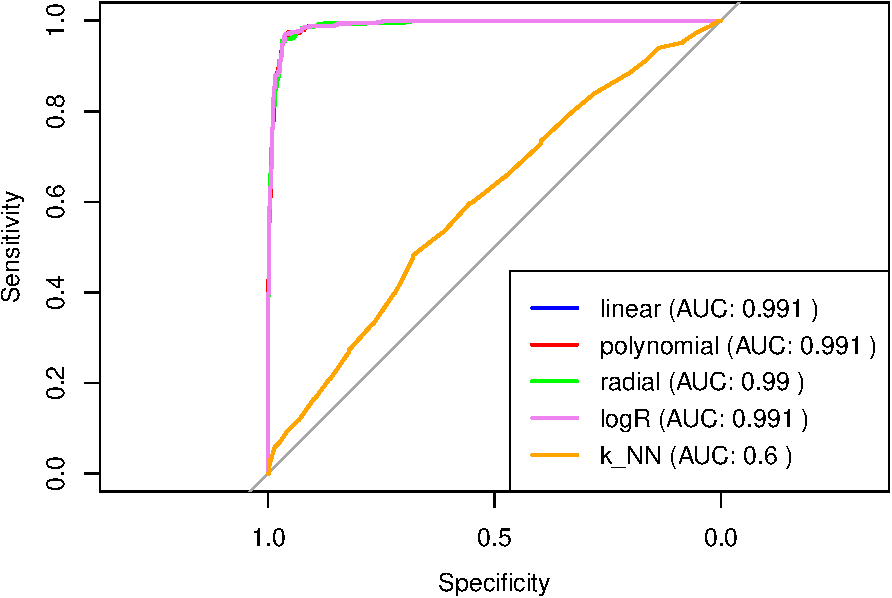
\includegraphics{Ergebnisse_files/figure-latex/S1ROC-1.pdf}
\caption{ROC-Kurven Szenario 1}
\label{fig:S1ROC}
\end{minipage}
\hfill
\begin{minipage}{0.48\linewidth}
\centering
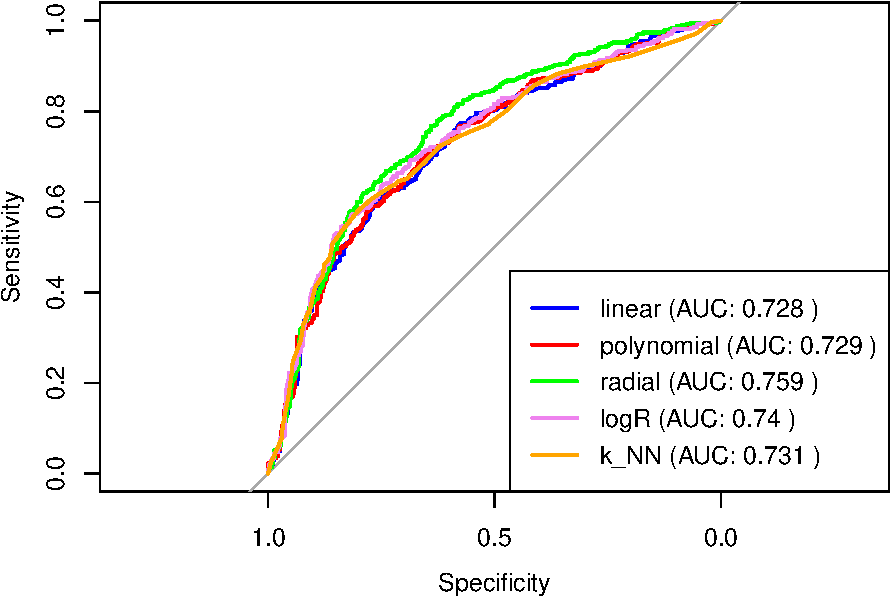
\includegraphics{Ergebnisse_files/figure-latex/S2ROC-1.pdf}
\caption{ROC-Kurven Szenario 2}
\label{fig:S2ROC}
\end{minipage}
\vspace*{0.5cm}\newline
\begin{minipage}{\linewidth}
\centering
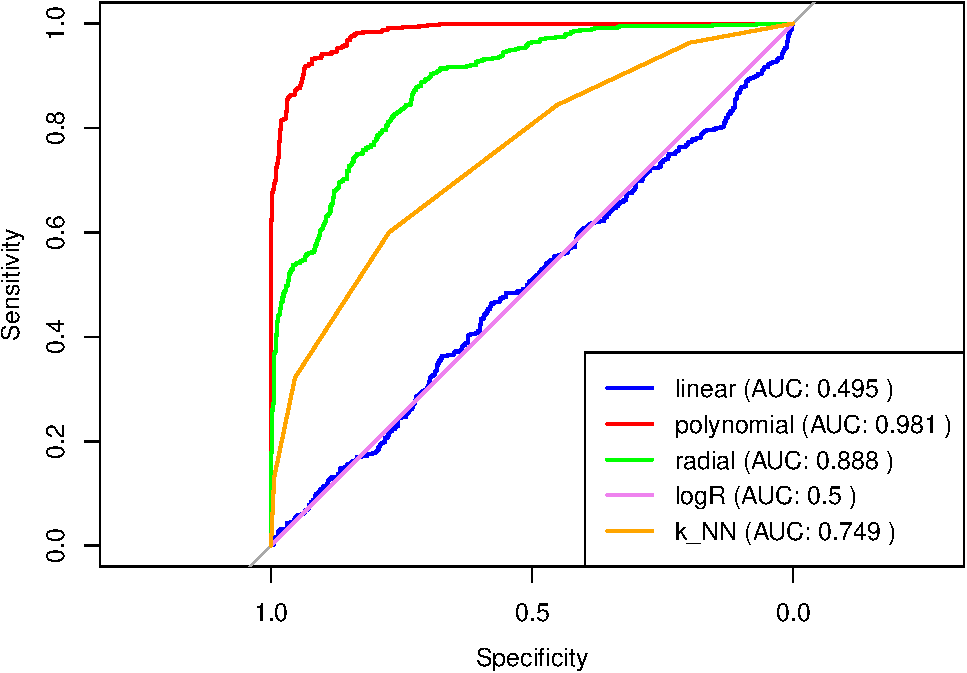
\includegraphics[width=0.48\linewidth]{Ergebnisse_files/figure-latex/S3ROC-1.pdf}
\caption{ROC-Kurven Szenario 3}
\label{fig:S3ROC}
\end{minipage}
\end{figure}

Zuletzt wird ein Vergleich der einzelnen Dimensionen über die drei
Formen der Entscheidungsgrenze gezogen. So ist für \(p \ll n\)
ersichtlich, dass insbesondere \textit{SVM-P} und \textit{SVM-R} über
alle drei Szenarien gute Leistung (insbesondere für S1 und S3 mit
mindestens 0.9 über alle Werte) zeigen. Das gleiche gilt, mit Ausnahme
der polynomialen Form der Entscheidungsgrenze, auch für \(p \approx n\),
wobei die Werte etwas niedriger bei 0.8 bis 0.9 liegen. In den
hochdimensionalen Szenarien \(p \gg n\) ist einzig \textit{SVM-P}
überzeugend, erneut ausgenommen der polynomialen Form der
Entscheidungsgrenze. \newpage

\addcontentsline{toc}{section}{Literatur}

\printbibliography

\end{document}
